\chapter{TINJAUAN PUSTAKA}
\label{chap:tinjauanpustaka}

% Ubah bagian-bagian berikut dengan isi dari tinjauan pustaka
\section{Hasil penelitian terdahulu}
\label{sec:roketluarangkasa}
Pada subbab berikut akan dijabarkan penelitian terdahulu.

\subsection{Deteksi Objek Menggunakan YOLO V3}
\label{subsec:deteksiobjekmenggunakanyolov3}

Penelitian oleh \emph{Wijaya et al.} (2022) berfokus pada pengembangan sistem deteksi objek yang menggunakan \emph{algoritma YOLO V3} untuk meningkatkan keamanan dalam sistem mobilitas. \emph{Algoritma YOLO V3} merupakan salah satu metode \emph{deep learning} yang dirancang untuk melakukan deteksi objek secara cepat dan akurat pada gambar atau video. Penelitian ini memanfaatkan \emph{YOLO V3} untuk mendeteksi rintangan yang ada di lingkungan sekitar sistem, sehingga dapat membantu dalam menghindari potensi bahaya yang diakibatkan oleh tabrakan dengan objek yang tidak terdeteksi.

Fitur utama dalam penelitian ini adalah implementasi \emph{YOLO V3} sebagai algoritma deteksi objek \emph{real-time}. Algoritma ini memiliki keunggulan dalam kecepatan dan akurasinya, memungkinkan sistem untuk mendeteksi berbagai objek dengan lebih cepat dibandingkan metode deteksi lainnya. \emph{YOLO V3} juga memungkinkan sistem untuk secara simultan mengenali beberapa objek dalam satu \emph{frame} gambar, yang sangat penting dalam lingkungan yang dinamis. Penelitian ini menekankan bahwa penggunaan \emph{YOLO V3} dapat secara signifikan meningkatkan keamanan sistem yang memerlukan deteksi objek secara \emph{real-time} \cite{wijaya2022deteksi}.

\subsection{Perancangan Sistem Kontrol Motor Kursi Roda}
\label{subsec:perancangansistemkontrolmotorkursiroda}

Penelitian yang dilakukan oleh \emph{Ekatama} (2024) membahas tentang perancangan sistem kontrol motor kursi roda yang dioperasikan secara nirkabel dengan menggunakan \emph{ESP32}. Dalam penelitian ini, \emph{ESP32} dimanfaatkan sebagai pusat kendali yang mampu mengatur pergerakan motor kursi roda tanpa menggunakan koneksi kabel. Penggunaan koneksi nirkabel ini memungkinkan pengendalian kursi roda dari jarak jauh melalui perangkat yang mendukung \emph{Wi-Fi} atau \emph{Bluetooth}, menawarkan kemudahan dan kenyamanan bagi pengguna dalam mengendalikan kursi roda mereka.

Fitur utama dari penelitian ini melibatkan penggunaan \emph{ESP32} sebagai platform utama untuk mengatur pergerakan motor kursi roda. \emph{ESP32} dipilih karena kemampuannya dalam menyediakan komunikasi nirkabel yang stabil dan efisien. Selain itu, penelitian ini menyoroti bagaimana sistem yang dirancang dapat beroperasi dengan konsumsi daya yang rendah, yang merupakan faktor penting dalam perangkat yang diharapkan memiliki masa penggunaan yang lama. Dengan demikian, sistem ini dioptimalkan untuk menjaga efisiensi daya tanpa mengorbankan kinerja atau responsivitas \cite{ekatama2024perancangan}.

\subsection{Deteksi Objek Berbasis ESP32-CAM}
\label{subsec:deteksiobjekberbasisesp32cam}

Penelitian yang dilakukan oleh \emph{Narwaria et al.} (2024) mengeksplorasi penggunaan \emph{ESP32-CAM} dalam mengembangkan sistem deteksi objek berbasis \emph{YOLO}. \emph{ESP32-CAM} adalah modul kamera yang dirancang untuk menangkap gambar secara efisien dan cocok untuk aplikasi \emph{Internet of Things (IoT)}. Penelitian ini menggunakan \emph{ESP32-CAM} bersama dengan algoritma \emph{YOLO} untuk mendeteksi dan mengenali objek secara \emph{real-time}. Sistem ini dirancang untuk menangani kebutuhan deteksi objek di berbagai aplikasi, seperti sistem pengawasan, pengenalan objek, dan visi komputer.

Fitur utama dari penelitian ini adalah kombinasi antara \emph{ESP32-CAM} dan \emph{algoritma YOLO}. \emph{ESP32-CAM} memberikan platform \emph{hardware} yang hemat daya dan biaya rendah, sementara \emph{YOLO} menyediakan kemampuan deteksi objek yang cepat dan akurat. Penelitian ini menunjukkan bahwa penggunaan \emph{Python} dan \emph{OpenCV} sebagai \emph{tools} dalam memrogram dan mengolah data visual memungkinkan sistem untuk menangani pemrosesan gambar dan deteksi objek dengan efisiensi yang tinggi. Solusi ini menunjukkan potensi besar dalam mengembangkan sistem deteksi objek untuk berbagai aplikasi \emph{real-time} \cite{10696374}.

\section{Object Detection}
\label{sec:detection}

\emph{Object detection} atau deteksi objek adalah teknologi inti dalam banyak aplikasi modern seperti sistem pengawasan, pengenalan wajah, dan kendaraan otonom. Teknologi ini digunakan untuk mendeteksi dan mengklasifikasikan berbagai objek dalam gambar atau video. Dalam konteks penelitian ini, \emph{object detection} berperan penting untuk mendeteksi keberadaan manusia sehingga kursi roda otonom dapat mengikuti gerakan pengguna secara real-time. Perkembangan pesat dalam \emph{deep learning}, terutama dengan penggunaan \emph{Convolutional Neural Network} (CNN), telah mengoptimalkan kemampuan \emph{object detection}. \emph{CNN}, dengan berbagai lapisannya seperti lapisan konvolusi, aktivasi, \emph{pooling}, dan \emph{fully connected}, menjadi fondasi dari banyak metode deteksi objek saat ini, termasuk \emph{YOLO} (You Only Look Once).

\emph{YOLO}, salah satu metode deteksi objek paling populer, mampu melakukan deteksi dengan kecepatan tinggi dan akurasi yang baik, menjadikannya sangat cocok untuk aplikasi \emph{real-time} seperti kursi roda otonom. \emph{YOLOv11}, versi terbaru dari keluarga \emph{YOLO}, menawarkan peningkatan signifikan dalam kecepatan dan akurasi, serta tambahan fitur seperti \emph{YOLO pose} untuk deteksi pose manusia. Selain itu, metode pelacakan objek seperti \emph{DeepSORT} yang menggunakan \emph{Kalman Filter} dan \emph{Hungarian Algorithm}, serta teknologi lainnya seperti \emph{MediaPipe Pose}, semakin memperkuat kemampuan sistem kursi roda otonom dalam melacak dan mengikuti gerakan manusia dengan presisi tinggi.

\section{Convolutional Neural Network (CNN)}
\label{sec:cnn}

\emph{Convolutional Neural Network} (CNN) adalah jenis jaringan saraf tiruan yang dirancang khusus untuk pengolahan data yang memiliki struktur grid, seperti gambar. CNN terdiri dari serangkaian lapisan yang bekerja sama untuk mengekstraksi dan menganalisis fitur dari data input, membuatnya sangat efektif dalam tugas-tugas seperti klasifikasi gambar, segmentasi, dan deteksi objek.

\subsection{Lapisan Konvolusi (\emph{Convolutional Layer})}
\label{subsec:Convolutional Layer}

Lapisan konvolusi adalah fondasi dari CNN yang bertugas mengekstraksi fitur-fitur penting dari input gambar. Dengan menerapkan filter yang dipelajari selama pelatihan, lapisan ini mampu mengenali elemen-elemen dasar seperti tepi, tekstur, dan pola dalam gambar. Setiap filter dalam lapisan konvolusi bertanggung jawab untuk mendeteksi fitur tertentu, dan hasilnya disusun dalam peta fitur (\emph{feature map}) yang memberikan representasi visual dari elemen-elemen yang terdeteksi. Formula untuk operasi konvolusi dapat dituliskan sebagai berikut:

\begin{equation}
  (f * g)(t) = \int_{-\infty}^{\infty} f(\tau)g(t - \tau) \, d\tau
\end{equation}

\subsection{Lapisan Aktivasi (\emph{Activation Layer})}
\label{subsec:Activation Layer}

Lapisan aktivasi adalah komponen yang menambahkan non-linearitas ke dalam jaringan, yang memungkinkan model untuk mempelajari hubungan yang lebih kompleks. Fungsi aktivasi seperti \emph{ReLU} (\emph{Rectified Linear Unit}) digunakan untuk mengaktifkan neuron hanya jika outputnya positif, sehingga mengurangi kompleksitas komputasi dan mempercepat proses pelatihan. Non-linearitas ini sangat penting untuk mengatasi masalah yang melibatkan data dengan struktur yang rumit, seperti deteksi objek dalam gambar.

\subsection{Lapisan \emph{Pooling} (\emph{Pooling Layer})}
\label{subsec:Pooling Layer}

Lapisan \emph{pooling} digunakan untuk mengurangi dimensi peta fitur sambil mempertahankan informasi yang paling relevan. Metode \emph{pooling} seperti \emph{max pooling} mengambil nilai maksimum dalam setiap area \emph{pooling}, yang membantu jaringan menjadi lebih tahan terhadap variasi kecil dalam input, seperti perubahan skala atau rotasi objek. Dengan mereduksi jumlah data yang harus diproses, \emph{pooling} juga membantu mengurangi risiko \emph{overfitting} dan mempercepat pelatihan. Operasi \emph{max pooling} dapat direpresentasikan sebagai:

\begin{equation}
  P(x, y) = \max_{i,j \in \mathrm{PoolRegion}} I(x+i, y+j)
\end{equation}

\subsection{Lapisan \emph{Fully Connected} (\emph{Fully Connected Layer})}
\label{subsec:Fully Connected Layer}

Lapisan \emph{fully connected} adalah lapisan terakhir dalam CNN yang menghubungkan setiap neuron di lapisan sebelumnya ke setiap neuron di lapisan ini. Lapisan ini berfungsi untuk menggabungkan semua fitur yang telah diekstraksi oleh lapisan konvolusi dan \emph{pooling}, dan menghasilkan output akhir, seperti prediksi kelas objek. Lapisan \emph{fully connected} memegang peran penting dalam memproses informasi yang dihasilkan dari lapisan-lapisan sebelumnya untuk membuat keputusan akhir tentang klasifikasi atau deteksi. Rumus dasar untuk operasi \emph{fully connected} dapat dituliskan sebagai:

\begin{equation}
  y = f\left(\sum_{i=1}^{n} w_i x_i + b\right)
\end{equation}

Dimana \( w_i \) adalah bobot, \( x_i \) adalah input, \( b \) adalah bias, dan \( f \) adalah fungsi aktivasi.

\section{Pose Estimation}
\label{sec:Pose Estimation}

\emph{Pose estimation} adalah teknik untuk mengidentifikasi dan melacak posisi tubuh manusia dalam gambar atau video. Teknik ini biasanya melibatkan deteksi titik-titik kunci (\emph{keypoints}) pada tubuh, seperti sendi atau ujung-ujung anggota tubuh, yang digunakan untuk memodelkan postur atau gerakan individu. \emph{Pose estimation} sangat penting dalam berbagai aplikasi, seperti analisis olahraga, animasi, dan interaksi manusia-mesin.

Dalam penelitian ini, \emph{pose estimation} digunakan untuk memastikan gerakan pengguna dapat diikuti dengan akurasi tinggi. Dengan memanfaatkan \emph{pose estimation}, sistem dapat memahami arah dan intensitas gerakan pengguna, yang memungkinkan kursi roda untuk merespons secara tepat dan efisien.

\section{YOLO (\emph{You Only Look Once})}
\label{sec:YOLO}

\emph{YOLO}, yang dikembangkan oleh Joseph Redmon, memperkenalkan pendekatan \emph{End-to-End} untuk deteksi objek dalam \emph{Real-Time}. Nama \emph{YOLO}, singkatan dari \emph{"You Only Look Once"} (Anda Hanya Melihat Sekali), mencerminkan kemampuan model ini dalam menyelesaikan tugas deteksi hanya dengan satu kali pemrosesan jaringan. Hal ini berbeda dengan pendekatan sebelumnya, yang menggunakan teknik \emph{sliding window} dan memerlukan pengklasifikasi yang harus dijalankan berkali-kali pada setiap gambar, atau metode lain yang memecah tugas menjadi dua langkah terpisah: pertama, mengidentifikasi daerah yang mungkin mengandung objek (\emph{region proposals}), dan kedua, menjalankan pengklasifikasi pada daerah yang telah diidentifikasi tersebut. Selain itu, \emph{YOLO} memanfaatkan \emph{output} yang lebih sederhana dengan hanya menggunakan regresi untuk memprediksi hasil deteksi, berlawanan dengan metode seperti \emph{Fast R-CNN} yang memisahkan tugas menjadi dua \emph{output} terpisah: probabilitas klasifikasi dan regresi untuk koordinat \emph{bounding box}.

\subsection{YOLOv8}
\label{subsec:YOLOv8}

\emph{YOLOv8} adalah salah satu model deteksi objek yang sangat efisien, menggabungkan kecepatan tinggi dengan akurasi yang relatif tinggi. Arsitektur ini terdiri dari beberapa lapisan utama: \emph{Backbone}, \emph{Neck}, dan \emph{Head}. \emph{Backbone} bertugas untuk mengekstraksi fitur-fitur dasar dari gambar input. Kemudian, \emph{Neck} menggabungkan informasi dari berbagai lapisan untuk menghasilkan representasi fitur yang lebih kaya, yang kemudian diproses oleh \emph{Head} untuk menghasilkan prediksi \emph{bounding box}, label kelas, dan skor \emph{confidence}.

\begin{figure}[H] 
  \centering 
  \includegraphics[scale=0.5]{gambar/YoloV8Architecture.jpg} 
  \caption{Arsitektur YOLOv8.} 
  \label{fig:ArsitekturYOLOv8} 
\end{figure}

Gambar menunjukkan arsitektur lengkap \emph{YOLOv8}, dimulai dari input gambar dengan resolusi 640x640x3, yang diproses melalui serangkaian lapisan konvolusi dalam \emph{Backbone} untuk mengekstraksi fitur penting. Kemudian, fitur-fitur ini diteruskan melalui \emph{Neck} yang menggabungkan dan mengolah informasi dari berbagai level resolusi, menghasilkan representasi multi-skala yang kaya. Akhirnya, \emph{Head} bertanggung jawab untuk melakukan prediksi akhir, seperti \emph{bounding boxes}, label kelas, dan \emph{confidence score}.

\emph{YOLOv8} memprediksi \emph{bounding box} menggunakan kombinasi antara koordinat pusat \((bx, by)\), dimensi \emph{bounding box} \((bw, bh)\), dan skor \emph{confidence} \(p_c\). Formula untuk menghitung koordinat \emph{bounding box} berdasarkan \emph{output} jaringan adalah:

\begin{equation}
  \begin{array}{c}
  bx = \sigma(t_x) + c_x\\
  bw = p_w e^{t_w}\\
  by = \sigma(t_y) + c_y\\ 
  bh = p_h e^{t_h}
  \end{array}
\end{equation}

Di mana \(t_x, t_y, t_w, t_h\) adalah \emph{output} dari model \emph{neural network}, \(\sigma\) adalah fungsi sigmoid, \(c_x, c_y\) adalah koordinat \emph{grid cell}, dan \(p_w, p_h\) adalah skala \emph{anchor box}.

Fungsi \emph{loss} dalam \emph{YOLOv8} terdiri dari beberapa komponen utama yang mengukur perbedaan antara prediksi model dan \emph{ground truth}, serta menyeimbangkan pentingnya prediksi koordinat, \emph{confidence score}, dan klasifikasi objek. Rumus fungsi \emph{loss}-nya adalah:

\begin{equation}
  \begin{array}{c}
  \mathbf{Loss} = \lambda_{\mathrm{coord}} \sum_{i=0}^{S^2} \sum_{j=0}^{B} \mathbb{1}_{ij}^{\mathrm{obj}} \left[ (bx_i - \hat{bx}_i)^2 + (by_i - \hat{by}_i)^2 \right] \\[10pt]
  + \lambda_{\mathrm{coord}} \sum_{i=0}^{S^2} \sum_{j=0}^{B} \mathbb{1}_{ij}^{\mathrm{obj}} \left[ (\sqrt{bw_i} - \sqrt{\hat{bw}_i})^2 + (\sqrt{bh_i} - \sqrt{\hat{bh}_i})^2 \right] \\[10pt]
  + \sum_{i=0}^{S^2} \sum_{j=0}^{B} \mathbb{1}_{ij}^{\mathrm{obj}} (C_i - \hat{C}_i)^2 + \lambda_{\mathrm{noobj}} \sum_{i=0}^{S^2} \sum_{j=0}^{B} \mathbb{1}_{ij}^{\mathrm{noobj}} (C_i - \hat{C}_i)^2 \\[10pt]
  + \sum_{i=0}^{S^2} \mathbb{1}_{i}^{\mathrm{obj}} \sum_{c \in \mathrm{classes}} (p_i(c) - \hat{p}_i(c))^2
  \end{array}
\end{equation}

Pada persamaan ini, \(S\) adalah ukuran grid, \(B\) adalah jumlah \emph{bounding boxes} per \emph{grid cell}, \(\mathbb{1}_{ij}^{\mathrm{obj}}\) adalah indikator bahwa \emph{bounding box} j di \emph{cell} i memprediksi objek, dan \(\lambda_{\mathrm{coord}}\) dan \(\lambda_{\mathrm{noobj}}\) adalah hyperparameter yang mengontrol pentingnya masing-masing \emph{loss}.
\newpage

\subsubsection{YOLOv8 Pose}
\label{subsubsec: YOLOv8 Pose}

\emph{YOLOv8 Pose} adalah varian dari \emph{YOLOv8} yang dirancang khusus untuk tugas \emph{pose estimation}. Dengan menggunakan pendekatan yang menggabungkan kecepatan \emph{YOLO} dengan kemampuan deteksi pose yang presisi, \emph{YOLOv8 Pose} mampu mendeteksi titik-titik kunci pada tubuh manusia secara \emph{real-time}. Setiap \emph{bounding box} tidak hanya mengandung informasi tentang lokasi dan ukuran objek, tetapi juga koordinat titik-titik kunci yang terkait dengan pose manusia (misalnya, bahu, siku, lutut, dan sebagainya).

\begin{figure}[H]
  \centering
  \includegraphics[scale=0.4]{gambar/yolov8Pose.png}
  \caption{YOLOv8 Pose.}
  \label{fig:Yolov8Pose}
\end{figure}

\subsection{YOLOv10}
\label{subsec:YOLOv10}

\emph{YOLOv10} merupakan pengembangan lebih lanjut dari \emph{YOLOv8}, dengan beberapa perbaikan dalam efisiensi dan akurasi deteksi objek. Seperti \emph{YOLOv8}, arsitektur \emph{YOLOv10} terdiri dari \emph{Backbone}, \emph{Neck}, dan \emph{Head}, namun dengan penambahan beberapa modul baru seperti \emph{Path Aggregation Network} (\emph{PSA}) dan \emph{Improved Convolutional Block} (\emph{C2fCIB}).

Arsitektur \emph{YOLOv10} dikembangkan dengan memperkenalkan beberapa peningkatan kunci dari dasar-dasar \emph{YOLOv8}. \emph{Backbone YOLOv10} tetap berfungsi sebagai ekstraktor fitur utama, namun ditingkatkan dengan modul \emph{SCD} (\emph{Squeeze-and-Excitation Convolutional Downsample}) dan \emph{C2fCIB}, yang memungkinkan propagasi informasi yang lebih efisien dan reduksi redundansi. Modul \emph{PSA} (\emph{Path Aggregation Network}) yang baru ditambahkan dalam \emph{Neck} membantu menggabungkan informasi dari berbagai jalur dalam jaringan, memperkaya representasi fitur untuk deteksi multi-skala.

\begin{figure}[H]
  \centering
  \includegraphics[scale=0.7]{gambar/YoloV10Architecture.png}
  \caption{Arsitektur YOLOv10.}
  \label{fig:ArsitekturYolov10}
\end{figure}

\subsection{YOLOv11}
\label{subsec:YOLOv11}

YOLO11 adalah terobosan terbaru dalam seri detektor objek real-time dari Ultralytics. Meneruskan kemajuan dari pendahulunya, YOLO11 menghadirkan peningkatan signifikan pada arsitekturnya, menjadikannya solusi yang kuat dan adaptif untuk berbagai aplikasi \emph{computer vision}. \emph{Ultralytics} memperkenalkan berbagai peningkatan dalam deteksi objek dan arsitektur pembelajaran mendalam. Arsitektur \emph{backbone} dan \emph{neck} yang ditingkatkan memperbaiki ekstraksi fitur, memungkinkan deteksi objek yang lebih akurat dan penanganan tugas yang lebih kompleks. 

Efisiensi dan kecepatan juga dipertajam melalui arsitektur yang disempurnakan dan \emph{pipeline} pelatihan yang lebih optimal, sehingga pemrosesan menjadi lebih cepat tanpa mengorbankan akurasi dan performa. \emph{YOLO11} mendukung implementasi di berbagai platform, mulai dari perangkat \emph{edge}, platform \emph{cloud}, hingga sistem dengan \emph{GPU NVIDIA}, membuatnya fleksibel untuk digunakan di berbagai lingkungan. Selain itu, \emph{YOLO11} mendukung beragam tugas, termasuk deteksi objek, segmentasi \emph{instance}, klasifikasi gambar, estimasi \emph{pose}, dan deteksi objek terorientasi (\emph{OBB}). Salah satu pembaruan utama dalam arsitektur \emph{YOLO11} adalah pengenalan modul \emph{C3K2} yang menggantikan modul \emph{C2F} pada \emph{YOLOv8}, serta penambahan modul \emph{C2PSA} setelah modul \emph{SPPF} untuk meningkatkan kapabilitas deteksi lebih lanjut.

\begin{figure}[H]
  \centering
  \resizebox{1\linewidth}{!}{
    \begin{tikzpicture}[node distance=1.5cm]
% Backbone Nodes
\node (input) [label] {Input};
\node (cbs0) [cbs, above of=input, yshift=1cm] {CBS\\k=3, s=2, p=1};
\node (cbs1) [cbs, above of=cbs0] {CBS\\k=3, s=2, p=1};
\node (c3k2_1) [c3k2, above of=cbs1] {C3K2\\C3k=Fa  lse};
\node (cbs2) [cbs, above of=c3k2_1] {CBS\\k=3, s=2, p=1};
\node (c3k2_2) [c3k2, above of=cbs2] {C3K2\\C3k=False};
\node (cbs3) [cbs, above of=c3k2_2] {CBS\\k=3, s=2, p=1};
\node (c3k2_3) [c3k2, above of=cbs3] {C3K2\\C3k=True};
\node (cbs4) [cbs, above of=c3k2_3] {CBS\\k=3, s=2, p=1};
\node (c3k2_4) [c3k2, above of=cbs4] {C3K2\\C3k=True};
\node (sppf) [layer, above of=c3k2_4, fill=green!20, align=center] {SPPF};
\node (c2psa) [layer, above of=sppf, fill=green!20, align=center] {C2PSA};

% Neck Nodes
\node (up1) [upsample, right of=sppf, xshift=2.25cm, minimum width=2cm] {Upsample};
\node (cc1) [concat, right of=up1, xshift=.5cm] {Concat};
\node (c3k2_5) [c3k2, right of=cc1, xshift=1cm] {C3K2\\C3k=False};

\node (up2) [upsample, below of=c3k2_5, minimum width=2cm] {Upsample};
\node (cc2) [concat, right of=up2, xshift=.5cm] {Concat};
\node (c3k2_6) [c3k2, right of=cc2, xshift=1cm] {C3K2\\C3k=False};

\node (cbs5) [cbs, above of=c3k2_6] {CBS\\k=3, s=2, p=1};
\node (cc3) [concat, right of=cbs5, xshift=1cm] {Concat};
\node (c3k2_7) [c3k2, right of=cc3, xshift=1cm] {C3K2\\C3k=False};

\node (cbs6) [cbs, above of=c3k2_7] {CBS\\k=3, s=2, p=1};
\node (cc4) [concat, right of=cbs6, xshift=1cm] {Concat};
\node (c3k2_8) [c3k2, right of=cc4, xshift=1cm] {C3K2\\C3k=True};

% Head Nodes
\node (detect1) [detect,  right of=c3k2_8, xshift=2cm] {Detect};
\node (detect2) [detect, below of=detect1] {Detect};
\node (detect3) [detect, below of=detect2] {Detect};

% SPPF Diagram
\node (cbs7) [cbs, right of=c3k2_3, xshift=4.75cm] {CBS \\ $k=1, s=1, p=1$};
\node (maxpool1) [layer, fill=red!30, below of=cbs7] {Maxpool};
\node (maxpool2) [layer, fill=red!30, below of=maxpool1] {Maxpool};
\node (maxpool3) [layer, fill=red!30, below of=maxpool2] {Maxpool};
\node (cc5) [concat, fill=blue!50, below of=maxpool3] {Concat};
\node (cbs8) [cbs, below of=cc5] {CBS \\ $k=1, s=1, p=1$};

% C2PSA Diagram
\node (cbs9) [cbs, right of=cbs7, xshift=4.75cm, yshift=.5cm] {CBS \\ $k=1, s=1, p=0$};
\node (split1) [layer, fill=cyan!30, below of=cbs9] {Split};
\node (PSA1) [layer, fill=purple!20, below of=split1] {PSABlock};
\node (dots) [label, below of=PSA1] {...};
\node (PSA2) [layer, fill=purple!20, below of=dots] {PSABlock};
\node (cc6) [concat, fill=blue!50, below of=PSA2] {Concat};
\node (cbs10) [cbs, below of=cc6] {CBS \\ $k=1, s=1, p=0$};

\node (attention) [layer, fill=cyan!30, right of=maxpool2, xshift=9.75cm] {Attention};
\node (cbs11) [cbs, below of=attention, yshift=-1.5cm] {CBS \\ $k=1, s=1, p=0$};
\node (cbs12) [cbs, below of=cbs11] {CBS \\ $k=1, s=1, p=0$};
\node (n1) [label, below of=cbs12] { };
\node (ffn) [label, above of=cbs11, xshift=-1cm, yshift=-.7cm] {FFN};
\node (h1) [label, above of=attention] { };

% CBS
\node (conv2d) [conv2D, right of=cbs9, minimum width=2cm, xshift=7.5cm] {Conv2D};
\node (bN) [layer, right of=conv2d, fill=orange!50, minimum width=1.5cm, xshift=.75cm] {BN};
\node (siLU) [layer, right of=bN, fill=yellow!50, minimum width=2cm, xshift=.75cm] {SiLU};

% Detection
\node (cbs22) [cbs, right of=PSA2, xshift=8cm] {CBS\\k=3, s=1, p=1};
\node (cbs21) [cbs, above of=cbs22] {CBS\\k=3, s=1, p=1};
\node (conv2d_1) [conv2D, below of=cbs22] {Conv2D};
\node (bbox) [layer, below of=conv2d_1, fill=red!50, minimum width=2cm,] {Bbox\\Loss};
\node (h2) [label, above of=cbs21] { };

\node (cbs31) [cbs, right of=cbs21, xshift=2cm] {CBS\\k=3, s=1, p=1};
\node (cbs32) [cbs, below of=cbs31] {CBS\\k=3, s=1, p=1};
\node (conv2d_2) [conv2D, below of=cbs32] {Conv2D};
\node (cls) [layer, below of=conv2d_2, fill=red!50, minimum width=2cm,] {Cls\\Loss};
\node (h3) [label, above of=cbs31] { };

% Labels
\node (Bone) [label, below of=cbs0, xshift=1.1cm] {Backbone};
\node (SPPF) [label, right of=Bone, xshift=5.1cm] {SPPF};
\node (C2PSA)[label, right of=SPPF, xshift=9.3cm] {C2PSA};
\node (PSABlock) [label, above of=C2PSA] {PSABlock};
\node (Detect) [label, right of=C2PSA, xshift=7.1cm] {Detect};
\node (CBS) [label, above of=Detect, yshift=8.3cm] {CBS};
\node (legend) [label, font=\small, left of=CBS, xshift=-2.8cm] {$kernel size(k), stride(s), padding(p)$};
\node (Head) [label, above of=CBS, yshift=1.2cm] {Head};
\node (Neck) [label, left of=Head, xshift=-1.7cm] {Neck};

% Blocks
\draw [dashed, thick, rounded corners] ($(cbs0.south west) - (.75,1.25)$) rectangle ($(c2psa.north east) + (.75,.75)$);
\draw [dashed, thick, rounded corners] ($(up1.south west) - (.25,2.25)$) rectangle ($(c3k2_8.north east) + (.25,.75)$);
\draw [dashed, thick, rounded corners] ($(detect3.south west) - (.75,.75)$) rectangle ($(detect1.north east) + (.75,.75)$);
\draw [dashed, thick, rounded corners] ($(conv2d.south west) - (.5,1)$) rectangle ($(siLU.north east) + (.75,.5)$);
\draw [dashed, thick, rounded corners] (2.5,.4) rectangle (8.5,12.75);
\draw [dashed, thick, rounded corners] (8.75,.4) rectangle (19.75,12.75);
\draw [dashed, thick, rounded corners] (15,1.9) rectangle (19.5,10);
\draw [dashed, thick, rounded corners] (20,.4) rectangle (27.75,10);

% Bracket for repeated layers
\draw [decorate, decoration={brace, amplitude=10pt}] 
    (14.2,9.5) -- (14.2,5) 
    node[midway, right=.3] {$n$};
\draw [decorate, decoration={brace, amplitude=10pt}] 
    ($(cbs21.north west)+(0,1)$) -- ($(cbs31.north east)+(0,1)$)
    node[midway, right=.3] { };

\draw [arrow] (maxpool1.west) -| +(-1.5,-1) |- (cc5);
\draw [arrow] (maxpool2.west) -| +(-1,-1) |- (cc5);
\draw [arrow] (maxpool3.west) -| +(-.5,-1) |- (cc5);
\draw [arrow] (split1.west) -| +(-1.5,-1) |- (cc6);
\draw [arrow] (PSA1.west) -| +(-1,-1) |- (cc6);
\draw [arrow] (PSA2.west) -| +(-.5,-1) |- (cc6);
\draw [arrow] (attention.south) |- +(0,-.5) -| ++(-2,0) |- ++(1,1.5) -| (attention.north);
\draw [arrow] (cbs12.south) |- +(0,-.5) -| ++(-2,0) |- ++(1,3.5) -| (cbs11.north);


% Arrows Backbone
\draw [arrow] (input) -- (cbs0);
\draw [arrow] (cbs0) -- (cbs1); 
\draw [arrow] (cbs1) -- (c3k2_1);
\draw [arrow] (c3k2_1) -- (cbs2);
\draw [arrow] (cbs2) -- (c3k2_2);
\draw [arrow] (c3k2_2) -- (cbs3);
\draw [arrow] (cbs3) -- (c3k2_3);
\draw [arrow] (c3k2_3) -- (cbs4);
\draw [arrow] (cbs4) -- (c3k2_4);
\draw [arrow] (c3k2_4) -- (sppf);
\draw [arrow] (sppf) -- (c2psa);

% Arrows Neck
\draw [arrow] (c3k2_3.east) -| +(.25,0) |- +(1,3.75) -| (cc1);
\draw [arrow] (c3k2_2.east) -| +(.5,0) |- +(1,5.25) -| (cc2);
\draw [arrow] (c3k2_5.north) |- +(1,.25) -| (cc3);
\draw [arrow] (c2psa.north) |- +(1,.25) -| (cc4);
\draw [arrow] (c2psa.north) |- +(1,.25) -| (up1);
\draw [arrow] (c3k2_5) -- (up2);
\draw [arrow] (c3k2_6) -- (cbs5);
\draw [arrow] (c3k2_7) -- (cbs6);

% Arrow Head
\draw [arrow] (c3k2_8) -- (detect1);
\draw [arrow] (c3k2_7) -- (detect2);
\draw [arrow] (c3k2_6) -- (detect3);

\draw [arrow] (cbs7) -- (maxpool1);
\draw [arrow] (maxpool1) -- (maxpool2);
\draw [arrow] (maxpool2) -- (maxpool3);
\draw [arrow] (maxpool3) -- (cc5);
\draw [arrow] (cc5) -- (cbs8);

\draw [arrow] (cbs9) -- (split1);
\draw [arrow] (split1) -- (PSA1);
\draw [arrow] (PSA1) -- (dots);
\draw [arrow] (dots) -- (PSA2);
\draw[arrow] (PSA2) -- (cc6);
\draw[arrow] (cc6) -- (cbs10);

\draw[arrow] (h1) -- (attention);
\draw[arrow] (attention) -- (cbs11);
\draw[arrow] (cbs11) -- (cbs12);
\draw[arrow] (cbs12) -- (n1);

\draw[arrow] (conv2d) -- (bN);
\draw[arrow] (bN) -- (siLU);

\draw[arrow] (h2) -- (cbs21);
\draw[arrow] (cbs21) -- (cbs22);
\draw[arrow] (cbs22) -- (conv2d_1);
\draw[arrow] (conv2d_1) -- (bbox);

\draw[arrow] (h3) -- (cbs31);
\draw[arrow] (cbs31) -- (cbs32);
\draw[arrow] (cbs32) -- (conv2d_2);
\draw[arrow] (conv2d_2) -- (cls);
\end{tikzpicture}
  }
  \caption{Arsitektur Yolov11}
  \label{fig:ArsitekturYolov11}
\end{figure}

Arsitektur \emph{C3K2} merupakan versi yang dimodifikasi dari modul \emph{C2F}. Perbedaan utama terletak pada konfigurasi parameter \emph{c3k}. Ketika \emph{c3k} disetel ke \texttt{False}, modul \emph{C3K2} berperilaku seperti modul \emph{C2F}, menggunakan struktur \emph{bottleneck} standar. Sebaliknya, ketika \emph{c3k} disetel ke \texttt{True}, modul \emph{bottleneck} digantikan oleh modul \emph{C3}. Perubahan ini dapat dilihat pada gambar berikut.

\begin{figure}[H]
  \centering
  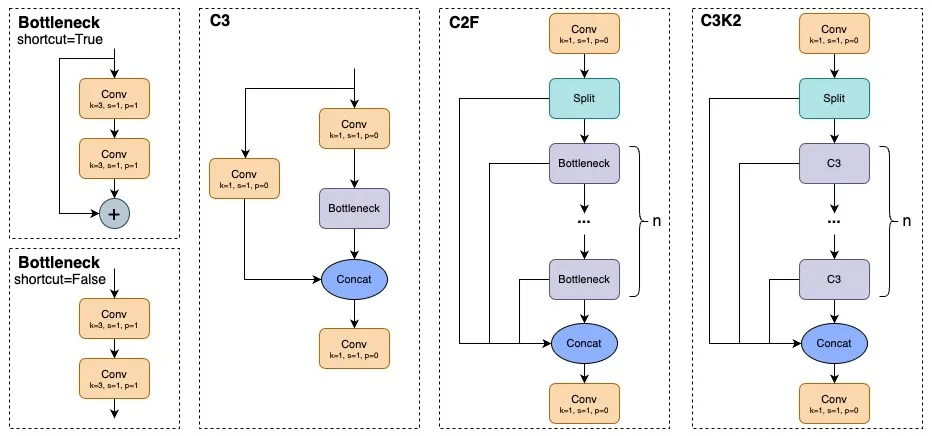
\includegraphics[scale=0.55]{gambar/C3k2.jpg}
  \caption{Modul Bottleneck, C3, C2F, dan C3K2}
  \label{fig:c3k2}
\end{figure}

Fitur input diubah pada lapisan \emph{feedforward} ke dalam ruang berdimensi lebih tinggi, sehingga hubungan non-linear yang kompleks dapat tertangkap dengan lebih stabil.

\section{MediaPipe}
\label{sec:MediaPipe}

\emph{MediaPipe} adalah framework \emph{open-source} yang dikembangkan oleh Google untuk membangun pipeline pemrosesan media yang efisien, termasuk dalam pengolahan gambar dan video. Framework ini menyediakan berbagai modul yang dapat dimanfaatkan untuk aplikasi seperti deteksi wajah, pelacakan tangan, dan estimasi pose.

Kerangka kerja \emph{MediaPipe} menggunakan konsep "graph," di mana setiap node dalam graph berfungsi sebagai "calculator" yang menjalankan tugas spesifik, seperti deteksi objek, pelacakan pose, atau segmentasi gambar. Konfigurasi node-node ini dapat disesuaikan melalui \emph{GraphConfig}, yang mendefinisikan topologi dan fungsionalitas dari keseluruhan sistem.

\begin{figure}[H]
  \centering
  \includegraphics[scale=0.5]{gambar/MediaPipe3D.png}
  \caption{MediaPipe 3D.}
  \label{fig:MediaPipe3D}
\end{figure}

Salah satu contoh penggunaan \emph{MediaPipe} yang paling dikenal adalah estimasi pose manusia menggunakan modul \emph{MediaPipe Pose}. Teknik ini mengombinasikan estimasi pose 2D dengan model humanoid yang lebih kompleks, serta menggunakan metode optimasi untuk menghitung sudut sendi dalam pose 3D. Pendekatan ini efektif dalam mengatasi masalah ambiguitas kedalaman pada estimasi pose 3D, dan mampu bekerja secara \emph{real-time}. Visualisasi pose 3D yang dihasilkan memperlihatkan setiap sendi tubuh sebagai titik dan garis penghubung antar sendi, memberikan gambaran yang jelas mengenai posisi dan orientasi tubuh di dalam ruang 3D.

\subsection{MediaPipe Pose}
\label{subsec:MediaPipe Pose}

\emph{MediaPipe Pose} adalah modul dalam \emph{MediaPipe} yang dirancang khusus untuk mendeteksi dan melacak pose manusia secara \emph{real-time}. Dengan menggunakan model \emph{machine learning} yang canggih, \emph{MediaPipe Pose} dapat mengidentifikasi hingga 33 titik referensi pada tubuh manusia, memungkinkan sistem untuk memahami dan merespons gerakan pengguna secara cepat dan akurat.

\begin{figure}[H]
  \centering
  \includegraphics[scale=0.5]{gambar/mp_pose.jpg}
  \caption{MediaPipe Pose.}
  \label{fig:mp_pose}
\end{figure}

\section{Classification Performance}
\label{sec:Classification Performance}

\emph{Classification performance} mengacu pada kemampuan model untuk mengklasifikasikan data input ke dalam kategori yang benar. Proses pengklasifikasian memerlukan evaluasi untuk menilai efektivitas model yang telah dikembangkan, biasanya dengan menggunakan set data pengetesan. Salah satu pendekatan evaluasi yang sering digunakan dalam konteks pengklasifikasian adalah \emph{confusion matrix}, yang memberikan visualisasi mengenai kinerja model dalam mengategorikan data secara akurat.

\begin{figure}[H]
  \centering
  \includegraphics[scale=0.5]{gambar/Matrix Konfusi.jpg}
  \caption{Matrix Konfusi.}
  \label{fig:confusion}
\end{figure}

\emph{Confusion matrix} ini digunakan untuk mengevaluasi kinerja model klasifikasi biner dan menampilkan empat jenis hasil dari prediksi model: \emph{True Positive} (TP), \emph{False Negative} (FN), \emph{False Positive} (FP), dan \emph{True Negative} (TN). TP terjadi ketika model memprediksi kelas positif dengan benar, sedangkan FN terjadi ketika model salah memprediksi kelas negatif padahal seharusnya positif (disebut juga sebagai \emph{Type II Error}). FP terjadi ketika model salah memprediksi kelas positif padahal seharusnya negatif (disebut juga sebagai \emph{Type I Error}), dan TN terjadi ketika model memprediksi kelas negatif dengan benar.

\section{Evaluation Metrics}
\label{sec:Evaluation Metrics}

Metrik evaluasi berfungsi sebagai dasar pemahaman dalam membandingkan efektivitas berbagai algoritma dan skenario yang berbeda. Melalui evaluasi yang teliti, perbandingan akurat antara berbagai teknik deteksi objek dapat dilakukan, serta tingkat keakuratan yang dicapai dapat dinilai dengan tepat. Hal ini menjadi sangat penting dalam pemilihan algoritma yang paling sesuai untuk tugas deteksi tertentu. Metrik seperti \emph{akurasi}, \emph{presisi}, dan \emph{recall} digunakan untuk mengevaluasi efektivitas model dalam mendeteksi dan mengidentifikasi objek dengan benar. Implementasi metrik-metrik ini diperlukan untuk menentukan model yang paling efisien.

Selain itu, analisis akurasi memberikan wawasan kuantitatif yang signifikan mengenai kinerja algoritma deteksi objek, serta detail lebih lanjut mengenai kemampuan algoritma dalam menghasilkan deteksi yang akurat. Kesalahan yang teridentifikasi melalui metrik evaluasi menjadi langkah penting dalam penelitian deteksi, seperti dalam kasus deteksi asap yang diteliti. Identifikasi ini memudahkan pemahaman mengenai potensi kesalahan dalam algoritma, yang kemudian dapat mengarah pada perbaikan dan peningkatan metode deteksi. Metrik evaluasi juga dimanfaatkan untuk mendukung pengoptimalan hiperparameter algoritma.

Dalam penelitian ini, berbagai metrik evaluasi seperti \emph{presisi}, \emph{recall}, dan \emph{Mean Average Precision} (mAP) telah diterapkan. Dengan menggabungkan metode evaluasi ini, penelitian ini dirancang untuk menyajikan analisis komprehensif mengenai kinerja algoritma deteksi objek yang ditinjau. Penjelasan mengenai konsep dasar metrik evaluasi akan dijabarkan sebagai berikut:

\subsection{Precision}
\label{subsec:precision}

\emph{Precision} merupakan salah satu metrik utama yang digunakan untuk mengukur seberapa akurat prediksi dari model terhadap objek yang terdeteksi. Metrik ini menunjukkan proporsi prediksi positif yang benar (\emph{True Positive}) dibandingkan dengan keseluruhan prediksi positif, baik yang benar (\emph{True Positive}) maupun salah (\emph{False Positive}), yang dinyatakan dengan persamaan berikut: 
\begin{equation} 
  \mathrm{Precision} = \frac{TP}{TP + FP} 
\end{equation}

Di mana \(TP\) (\emph{True Positive}): Prediksi benar, yaitu deteksi objek yang sesuai dengan \emph{ground truth} dan \(FP\) (\emph{False Positive}): Prediksi salah, yaitu deteksi objek yang tidak sesuai dengan \emph{ground truth}.

\emph{Precision} sangat berguna dalam situasi di mana kesalahan prediksi positif (\emph{false positive}) harus diminimalkan. Contohnya, dalam aplikasi kursi roda otonom, deteksi yang salah terhadap manusia dapat menyebabkan tindakan yang berbahaya, sehingga \emph{precision} harus dipertahankan pada nilai yang tinggi.

\emph{Precision} biasanya dikombinasikan dengan metrik lain, seperti \emph{recall}, untuk memberikan gambaran yang lebih lengkap tentang kinerja model.

\subsection{Recall}
\label{subsec:recall}

\emph{Recall} atau sensitivitas mengukur kemampuan model dalam mendeteksi semua objek yang ada pada gambar atau video. \emph{Recall} menekankan pada seberapa banyak objek yang benar-benar ada dalam data (\emph{ground truth}) yang berhasil terdeteksi oleh model dengan persamaan berikut:

\begin{equation} 
  \mathrm{Recall} = \frac{TP}{TP + FN} 
\end{equation}

Di mana \(TP\) (\emph{True Positive}): Prediksi benar, yaitu objek yang terdeteksi dengan benar dan \(FP\) (\emph{False Negative}): Prediksi salah, yaitu objek yang ada tetapi tidak terdeteksi.

Metrik ini penting ketika kesalahan berupa kegagalan dalam mendeteksi objek (\emph{false negative}) harus diminimalkan. Dalam konteks pengembangan kursi roda otonom, \emph{recall} sangat penting karena objek seperti manusia harus selalu terdeteksi agar kursi roda dapat mengikuti secara akurat.

\textbf{\emph{Trade-off Precision dan Recall:}} Dalam banyak kasus, \emph{precision} dan \emph{recall} memiliki hubungan yang berlawanan. Jika model terlalu konservatif dalam membuat prediksi, \emph{precision} akan tinggi, tetapi \emph{recall} rendah. Sebaliknya, jika model terlalu longgar dalam mendeteksi objek, \emph{recall} tinggi tetapi \emph{precision} menurun. Oleh karena itu, diperlukan keseimbangan antara \emph{precision} dan \emph{recall}, yang biasanya diekspresikan melalui metrik lain seperti \emph{F1-score}.

\subsection{Mean Average Precision (mAP)}
\label{subsec:mAP}

\emph{Mean Average Precision} (mAP) merupakan metrik komprehensif yang digunakan untuk mengukur performa model deteksi objek secara keseluruhan. \emph{mAP} adalah rata-rata dari \emph{average precision} (AP) di berbagai kelas yang ada dalam dataset.

\begin{equation} 
  \mathrm{AP} = \int_0^1 P(r) , dr 
\end{equation}

Di mana \(P(r)\) : \emph{Precision} sebagai fungsi dari \emph{recall} dan \(dr\) : Diferensial dari \emph{recall}.

AP dihitung dengan mencari area di bawah kurva \emph{precision-recall} (\emph{PR curve}) untuk setiap kelas. Setelah AP untuk semua kelas dihitung, rata-rata dari nilai-nilai tersebut akan memberikan nilai \emph{mAP}.

\begin{equation} 
  \mathrm{mAP} = \frac{1}{N} \sum_{i=1}^{N} \mathrm{AP}_i 
\end{equation}

Di mana \(N\) : Jumlah kelas dalam dataset dan \(AP_i\) : \emph{Average precision} untuk kelas ke-i.

\emph{mAP} memberikan gambaran yang lebih luas mengenai performa detektor objek, karena metrik ini mempertimbangkan baik \emph{precision} maupun \emph{recall} secara bersamaan. Nilai \emph{mAP} ini akan menjadi acuan untuk mengevaluasi performa sistem, seperti mendeteksi berbagai objek seperti manusia, rintangan, dan lingkungan sekitar.

\subsection{Intersection over Union (IoU)}
\label{subsec:IoU}

\emph{Intersection over Union} (\emph{IoU}) adalah metrik yang digunakan untuk mengevaluasi keakuratan deteksi posisi objek yang dilakukan oleh model dalam pemrosesan gambar. Area persinggungan antara kotak deteksi yang dihasilkan oleh model dan kotak referensi, yang dikenal sebagai \emph{Ground Truth}, dihitung untuk menilai kinerja model. Rasio ini diperoleh dengan membandingkan luas area irisan dari kedua kotak tersebut terhadap total luas area gabungan yang mereka cakup. Jika kedua kotak tersebut diperlakukan sebagai satu kesatuan, maka \emph{IoU} memberikan skor yang menunjukkan seberapa akurat model dalam memprediksi lokasi objek yang sebenarnya. Nilai \emph{IoU} akan semakin tinggi seiring dengan bertambahnya proporsi area persinggungan relatif terhadap keseluruhan area gabungan.

\begin{figure}[H]
  \centering
  \includegraphics[scale=0.27]{gambar/IoU bbox.jpg}
  \caption{Intersection over Union.}
  \label{fig:IoU bbox}
\end{figure}

Kinerja model deteksi objek dilakukan evaluasi kinerja model deteksi objek dengan cara membandingkan area tumpang tindih antara \emph{bounding box} prediksi dan \emph{bounding box} \emph{ground truth}. Nilai \emph{IoU} berkisar antara 0 hingga 1, di mana nilai yang lebih mendekati 1 menunjukkan tingkat akurasi yang lebih tinggi dalam deteksi dan penentuan lokasi objek.

Dalam proses evaluasi, \emph{bounding box} yang dihasilkan oleh model dibandingkan dengan \emph{bounding box ground truth}, yang ditentukan secara manual sebagai lokasi sebenarnya dari objek dalam citra. Perhitungan \emph{IoU} dilakukan dengan membagi luas area tumpang tindih antara kedua \emph{bounding box} tersebut dengan luas total area gabungan dari keduanya. Persamaan berikut digunakan untuk menghitung nilai \emph{IoU}: 

\begin{equation}
  IoU = \frac{\left |A\bigcap B  \right |}{\left | A\bigcup B \right |}.
\end{equation}

\emph{IoU} dipilih sebagai alat ukur karena kemampuannya untuk memberikan penilaian yang jelas tentang seberapa akurat model dalam mengidentifikasi dan membatasi objek di berbagai kondisi, termasuk variasi ukuran, orientasi, dan konteks objek dalam citra. Nilai \emph{IoU} yang lebih tinggi diindikasikan sebagai tanda bahwa model dapat diandalkan dalam mendeteksi dan mengidentifikasi objek dengan tingkat presisi yang tinggi.

\section{Tinjauan Pustaka BoT-SORT}

BoT-SORT merupakan salah satu metode multi-object tracking (MOT) yang dikembangkan dengan pendekatan tracking-by-detection. Pada prinsipnya, metode ini memanfaatkan beberapa teknik dari berbagai algoritma sebelumnya, terutama ByteTrack, untuk menyajikan pelacakan yang lebih canggih. Perbaikan pada metode ini bertujuan untuk meningkatkan kinerja pelacakan dalam lingkungan dinamis maupun statis dengan memperbaiki beberapa komponen utama, yang akan dijabarkan sebagai berikut \parencite{aharon2022botsortrobustassociationsmultipedestrian}:

\subsection{Kalman Filter}

Kalman Filter (KF) berfungsi untuk memprediksi lokasi objek di frame berikutnya berdasarkan pergerakan sebelumnya. BoT-SORT menggunakan KF dengan vektor status yang mencakup koordinat pusat objek ($x_c$, $y_c$), lebar ($w$), tinggi ($h$), dan laju perubahan (kecepatan) dari variabel-variabel tersebut ($\dot{x_c}$, $\dot{y_c}$, $\dot{w}$, $\dot{h}$) \parencite{bewley2016simple, wojke2017simple}. Vektor status ini didefinisikan sebagai:

\begin{equation}
  \begin{split}
    \vb*{x}_k = [x_{c}{\scriptstyle(k)}, y_{c}{\scriptstyle(k)}, w{\scriptstyle(k)}, h{\scriptstyle(k)}, \\        
    \dot{x_{c}}{\scriptstyle(k)}, \dot{y_{c}}{\scriptstyle(k)}, \dot{w}{\scriptstyle(k)}, \dot{h}{\scriptstyle(k)}]^\top
  \end{split}
\end{equation}

\begin{equation}
  \vb*{z}_k = [z_{x_c}{\scriptstyle(k)}, z_{y_c}{\scriptstyle(k)}, z_{w}{\scriptstyle(k)}, z_{h}{\scriptstyle(k)}]^\top
\end{equation}

Matriks noise proses ($\mathbf{Q}_k$) dan noise pengukuran ($\mathbf{R}_k$) disesuaikan agar lebih sensitif terhadap perubahan dalam frame, yang membantu meningkatkan akurasi pelacakan. Matriks $\mathbf{Q}_k$ dan $\mathbf{R}_k$ ditentukan sebagai berikut:

\begin{equation}
  \begin{split}
    \vb*{Q}_k = diag\big{(} (\sigma_{p} \hat{w}_{k-1|k-1})^2, (\sigma_{p} \hat{h}_{k-1|k-1})^2, \\
    (\sigma_{p} \hat{w}_{k-1|k-1})^2, (\sigma_{p} \hat{h}_{k-1|k-1})^2, \\
    (\sigma_{v} \hat{w}_{k-1|k-1})^2, (\sigma_{v} \hat{h}_{k-1|k-1})^2, \\ 
    (\sigma_{v} \hat{w}_{k-1|k-1})^2 ,(\sigma_{v} \hat{h}_{k-1|k-1})^2\big{)}
  \end{split}
\end{equation}

\begin{equation}
  \begin{split}
      \vb*{R}_k = diag\big{(}(\sigma_{m} \hat{w}_{k|k-1})^2, (\sigma_{m} \hat{h}_{k|k-1})^2, \\
      (\sigma_{m} \hat{w}_{k|k-1})^2, (\sigma_{m} \hat{h}_{k|k-1})^2\big{)} 
  \end{split}
\end{equation}

Dengan adanya perubahan ini, prediksi \emph{bounding box} lebih akurat dibandingkan dengan metode Kalman Filter tradisional, terbukti dengan peningkatan nilai HOTA (Higher Order Tracking Accuracy).

\begin{figure}[H]
  \centering
  \includegraphics[scale=0.3]{gambar/KF_width.png}
  \caption{Kalman Filter bbox.}
  \label{fig:KF width}
\end{figure}

Visualisasi bentuk \emph{bounding box} dibandingkan dengan \emph{Kalman filter} yang banyak digunakan~\parencite{wojke2017simple} (biru putus-putus) dan \emph{Kalman filter} yang diusulkan (hijau). Tampak bahwa lebar \emph{bounding box} yang dihasilkan oleh \emph{Kalman filter} yang diusulkan lebih sesuai dengan objek. \emph{Bounding box} biru putus-putus memotong bagian kaki objek (dalam merah), sedangkan \emph{bounding box} hijau mencapai lebar yang diinginkan.

\subsection{\emph{Camera Motion Compensation} (CMC)}

Pelacak berbasis tracking-by-detection seringkali mengalami masalah ID switch atau false negatives akibat gerakan kamera, terutama dalam situasi dinamis. BoT-SORT mengimplementasikan teknik kompensasi gerakan kamera (Camera Motion Compensation) dengan memanfaatkan affine transformation untuk menghitung transformasi antara dua frame. Dengan melakukan ekstraksi keypoints gambar ~\cite{shi1994good}, kemudian menggunakan sparse optical flow ~\cite{Bouguet1999PyramidalIO} untuk pelacakan fitur dengan penolakan outlier lokal berbasis translasi. Matriks affine $\vb*{A}_{k-1}^k\in \mathbb{R}^{2 \times 3}$ diselesaikan menggunakan metode RANSAC ~\cite{fischler1981random}. Penggunaan teknik pendaftaran spars memungkinkan pengabaian objek dinamis dalam adegan berdasarkan deteksi, sehingga memiliki potensi untuk memperkirakan gerakan latar belakang dengan lebih akurat.

\begin{equation}
  \begin{aligned}
      & \vb*{A}_{k-1}^k = 
      \begin{bmatrix}
          \vb*{M}_{2x2} | \vb*{T}_{2x1}
      \end{bmatrix} = 
      \begin{bmatrix}
          a_{11}\;a_{12}\;a_{13} \\ a_{21}\;a_{22}\;a_{23} \\ 
      \end{bmatrix}
  \end{aligned}
\end{equation}
\begin{equation}
  \begin{aligned}
  {
      \vb*{\tilde{M}}}^k_{k-1} = 
      \begin{bmatrix}
      \vb*{M} & \vb*{0} & \vb*{0} & \vb*{0} \\
      \vb*{0} & \vb*{M} & \vb*{0} & \vb*{0} \\
      \vb*{0} & \vb*{0} & \vb*{M} & \vb*{0} \\
      \vb*{0} & \vb*{0} & \vb*{0} & \vb*{M}
      \end{bmatrix}, \; 
      \tilde{\vb*{T}}_{k-1}^k = 
      \begin{bmatrix}a_{13}\\a_{23}\\ 0\\ 0\\ \vdots \\ 0\end{bmatrix}
  \end{aligned}
\end{equation}
\begin{equation}
  \begin{aligned}
      \hat{\vb*{x}}^\prime_{k|k-1} = \tilde{\vb*{M}}_{k-1}^k \hat{\vb*{x}}_{k|k-1} + \tilde{\vb*{T}}_{k-1}^k \\
  \end{aligned}
\end{equation}
\begin{equation}
    {{\vb*{P}}}^{\prime}_{k|k-1} = 
    \tilde{\vb*{M}}_{k-1}^k {\vb*{P}}_{k|k-1} {\tilde{\vb*{M}}_{k-1}}^{k^\top}
    \label{eq:cmc_cov}        
\end{equation}

Dimana $\vb*{M}\in \mathbb{R}^{2 \times 2}$ merupakan matriks yang berisi skala dan rotasi dari matriks afine $\vb*{A}$, dan $T$ mengandung komponen translasi. Trik matematis digunakan dengan mendefinisikan $\tilde{\vb*{M}}^k_{k-1}\in \mathbb{R}^{8 \times 8}$ dan $\tilde{\vb*{T}}_{k-1}^k\in \mathbb{R}^{8}$. Selanjutnya, $\hat{\vb*{x}}_{k|k-1}$ dan $\hat{\vb*{x}}^\prime_{k|k-1}$ didefinisikan sebagai vektor status prediksi dari Kalman Filter (KF) pada waktu $k$, sebelum dan setelah kompensasi gerakan kamera, sedangkan $\vb*{P}_{k|k-1}$ dan $\vb*{P'}_{k|k-1}$ didefinisikan sebagai matriks kovarians KF sebelum dan setelah koreksi. Setelah itu, $\hat{\vb*{x}}^\prime_{k|k-1}$ dan ${{\hat{\vb*{P}}}^{\prime}}_{k|k-1}$ digunakan dalam langkah update Kalman Filter sebagai berikut.

\begin{equation}
  \begin{aligned}
  & \vb*{K_k} =  {{\vb*{P}}}^{\prime}_{k|k-1} \vb*{H}_k^\top (\vb*{H}_k  {{\vb*{P}}}^{\prime}_{k|k-1} \vb*{H}_k^\top + \vb*{R}_k)^{-1} \\
  & \hat{\vb*{x}}_{k|k} = \hat{\vb*{x}}^\prime_{k|k-1} + \vb*{K}_k (\vb*{z}_k - \vb*{H}_k \hat{\vb*{x}}^\prime_{k|k-1}) \\
  & \vb*{P}_{k|k} = (\vb*{I}- \vb*{K}_k \vb*{H}_k)  {{\vb*{P}}}^{\prime}_{k|k-1}
  \end{aligned}
  \label{eq:cmc_update_kf}
\end{equation} 
`'
Dalam skenario kecepatan tinggi, koreksi penuh terhadap vektor status, termasuk komponen kecepatan, sangat penting. Jika kamera berubah dengan lambat dibandingkan dengan kecepatan frame, koreksi pada persamaan \ref{eq:cmc_cov} dapat diabaikan. Setelah mengompensasi gerakan kamera yang rigid dan dengan asumsi posisi objek hanya sedikit berubah dari satu frame ke frame berikutnya, pada aplikasi dengan frame rate tinggi, ketika deteksi hilang, prediksi lintasan dapat dilakukan menggunakan langkah prediksi KF, yang memungkinkan tampilan lintasan yang lebih kontinu dan MOTA yang lebih tinggi.

Visualisasi prediksi \emph{bounding box} (BB) dari tracklet digunakan untuk asosiasi dengan BB deteksi baru berdasarkan kriteria IoU maksimum. (a.1) dan (b.1) memperlihatkan prediksi dari Kalman Filter (KF). (a.2) dan (b.2) memperlihatkan prediksi dari KF setelah kompensasi gerakan kamera. Pada gambar (b.1), diperlihatkan skenario di mana pengabaian gerakan kamera dapat menyebabkan IDSWs atau FN. Sebaliknya, pada gambar (b.2), prediksi telah sesuai dengan lokasi yang diinginkan dan asosiasi berhasil dilakukan. Gambar \ref{fig:cmc} dihasilkan dari sekuens MOT17 \cite{milan2016mot16}, yang mencakup pergerakan kamera akibat manuver kendaraan yang berbelok ke arah kanan.

\begin{figure}[H]
  \centering
  \includegraphics[scale=0.35]{gambar/cmc_pred.png}
  \label{fig:cmc}
  \caption{Kompensasi Gerakan Kamera}
\end{figure}

\subsection{Fusi IoU - Re-ID}

Fitur Re-ID diintegrasikan untuk memanfaatkan kemajuan dalam representasi visual objek. Fitur Re-ID diekstraksi menggunakan FastReID dengan backbone ResNeSt50 \parencite{he2020fastreid, zhang2020resnest}, dan mekanisme exponential moving average (EMA) digunakan untuk memperbarui status appearance tracklet \parencite{wang2020towards}. Pembaruan status appearance dilakukan dengan rumus:

\begin{equation}
e_i^k = \alpha e_i^{k-1} + (1 - \alpha) f_i^k
\end{equation}

Di mana $e_i^k$ adalah status appearance untuk tracklet ke-$i$ pada frame $k$, $f_i^k$ adalah embedding appearance deteksi saat ini, dan $\alpha=0.9$ adalah momentum term.

Penggabungan antara informasi gerakan (IoU) dan appearance (cosine similarity) dilakukan dengan cara berikut. Pertama, kandidat dengan kesamaan cosinus rendah atau yang terlalu jauh berdasarkan skor IoU ditolak. Selanjutnya, nilai minimum pada setiap elemen matriks digunakan sebagai nilai akhir dari \emph{cost matrix} $C$. Pipeline fusi IoU-ReID ini dapat diformulasikan sebagai berikut:

\begin{equation}
    \begin{aligned}
    \hat{d}_{i, j}^{cos} = 
        \begin{cases}
                0.5 \cdot d_{i, j}^{cos}, \text{($d_{i, j}^{cos} < \theta_{emb})$ $\land$ $(d_{i, j}^{iou} < \theta_{iou})$}\\
            1, \text{otherwise}
        \end{cases}
    \end{aligned}
    \quad\quad C_{i, j} = \min\{d_{i, j}^{iou}, \hat{d}_{i, j}^{cos}\}    
    \label{eq:min_dist}        
\end{equation}

\begin{equation}
  \begin{aligned}
  \hat{b} = 
      \begin{cases}
          0, \quad\quad \Delta data \neq 0 \\
          1, \quad \neg ( \hat{t} \in [0, t] \lor b ) \\
          b, \quad\quad \text{otherwise}\\
      \end{cases}
  \end{aligned}       
\end{equation}

Di mana $C_{i, j}$ merupakan elemen $(i, j)$ dari \emph{cost matrix} $C$. $d_{i, j}^{iou}$ adalah jarak IoU antara prediksi \emph{bounding box} tracklet ke-$i$ dan \emph{bounding box} deteksi ke-$j$, yang merepresentasikan \emph{cost} gerakan. $d_{i, j}^{cos}$ adalah jarak cosinus antara deskriptor penampilan rata-rata tracklet ke-$i$ dan deskriptor deteksi baru ke-$j$. $\hat{d}_{i, j}^{cos}$ adalah \emph{cost} penampilan baru yang digunakan. $\theta_{iou}$ adalah \emph{threshold} kedekatan, yang ditetapkan sebesar 0.5, untuk menolak pasangan tracklet dan deteksi yang tidak mungkin. $\theta_{emb}$ adalah \emph{threshold} penampilan, yang digunakan untuk memisahkan asosiasi positif dari keadaan penampilan tracklet dan vektor embedding deteksi dari asosiasi negatif.
Permasalahan penugasan linear dari deteksi dengan \emph{confidence} tinggi, yaitu langkah asosiasi pertama, diselesaikan menggunakan algoritma Hungarian~\cite{kuhn1955hungarian} dan berdasarkan \emph{cost matrix} $C$, yang dibentuk menggunakan Persamaan~\ref{eq:min_dist}.

\section{\emph{RoboFlow}}
\label{sec:RoboFlow}

\emph{RoboFlow} adalah platform yang mendukung pengolahan data secara efisien dan efektif. Melalui berbagai fitur yang disediakan, mulai dari anotasi data hingga evaluasi model, \emph{RoboFlow} memastikan bahwa setiap tahap dalam alur kerja pembelajaran mesin dapat dilakukan dengan lebih terstruktur dan mudah diintegrasikan dengan kerangka kerja yang ada. Peningkatan kinerja model dapat dikembangkan tanpa terbebani oleh kompleksitas teknis dalam penyiapan data.

\begin{figure}[H]
  \centering
  \includegraphics[scale=0.3]{gambar/roboflow.jpg}
  \caption{Interface RoboFlow}
  \label{fig:roboflow}
\end{figure}

\emph{RoboFlow} memfasilitasi proses penandaan gambar melalui alat bantu intuitif, sehingga percepatan dalam pembuatan label untuk \emph{dataset} dapat tercapai. Gambar dalam \emph{dataset} secara otomatis dimodifikasi melalui augmentasi data untuk menciptakan variasi guna meningkatkan \emph{robustness} model yang dilatih. Dukungan untuk konversi antara berbagai format \emph{dataset} populer juga disediakan, memudahkan persiapan data untuk berbagai algoritma pembelajaran mesin. Selain itu, fungsi untuk membagi \emph{dataset} menjadi set pelatihan, validasi, dan pengujian untuk validasi model.

\emph{RoboFlow} juga menawarkan integrasi dengan banyak kerangka kerja pembelajaran mesin populer seperti \emph{TensorFlow}, \emph{PyTorch}, dan \emph{YOLO}, yang mencakup:

\begin{itemize}
    \item \emph{Ekspor Data}: \emph{Dataset} dapat dengan mudah diekspor dalam format yang siap digunakan oleh kerangka kerja pembelajaran mesin.
    \item \emph{Pelatihan Model}: Platform ini memungkinkan pelatihan model secara langsung menggunakan \emph{dataset} yang telah disiapkan dan dioptimalkan.
    \item \emph{Evaluasi Model}: Kinerja model diukur menggunakan metrik yang membantu dalam memahami dan menyesuaikan efektivitas model sesuai kebutuhan.
\end{itemize}

\section{OBS Studio}
\label{sec:OBS Studio}

\emph{OBS Studio} adalah perangkat lunak \emph{open-source} yang dirancang untuk streaming dan perekaman video. Dalam proyek ini, \emph{OBS Studio} digunakan untuk mendokumentasikan dan menganalisis performa kursi roda otonom selama fase pengujian. Perangkat lunak ini memungkinkan pemilihan berbagai sumber video input, termasuk \emph{webcam}, yang digunakan untuk merekam seluruh proses pengujian secara visual. Dengan \emph{OBS Studio}, proses pengujian dari awal hingga akhir dapat direkam secara lengkap, memungkinkan pengumpulan data visual yang kaya dan mendetail.

\begin{figure}[H]
  \centering
  \includegraphics[scale=0.22]{gambar/OBSStudio.png}
  \caption{Interface OBS Studio}
  \label{fig:Gambar OBS}
\end{figure}

\section{ESP32 Devkit V1}
\label{sec:ESP32 Devkit V1}

\emph{ESP32 Devkit V1} adalah sebuah mikrokontroler yang dilengkapi dengan kemampuan komunikasi nirkabel, termasuk \emph{Wi-Fi} dan \emph{Bluetooth}. Dalam proyek ini, \emph{ESP32 Devkit V1} digunakan sebagai modul komunikasi utama untuk kursi roda otonom. Perangkat ini memungkinkan kursi roda untuk berinteraksi dengan perangkat eksternal seperti \emph{smartphone} atau komputer melalui jaringan nirkabel.

Salah satu keunggulan utama dari \emph{Devkit} ini adalah banyaknya pin yang dimiliki, yang memungkinkan mikrokontroler untuk diprogram dengan berbagai tugas. Pin-pin ini memberikan fleksibilitas yang tinggi dalam menghubungkan berbagai sensor dan aktuator yang diperlukan. Dengan memanfaatkan berbagai pin tersebut, sistem dapat menjalankan beberapa tugas secara simultan, seperti mengumpulkan data dari sensor, mengontrol motor, dan mengelola komunikasi nirkabel.

\begin{figure}[H]
  \centering
  \includegraphics[scale=0.2]{gambar/ESP32-DEVKIT-V1-board.png}
  \caption{Gambar ESP32 Devkit V1}
  \label{fig:Gambar ESP32Devkit V1}
\end{figure}

\emph{Devkit} ini kompatibel dengan \emph{Arduino IDE} dengan bahasa pemrograman \emph{C++}, yang merupakan platform yang umum digunakan. \emph{Arduino IDE} menyediakan berbagai \emph{library} dan dukungan yang memudahkan proses pemrograman \emph{ESP32} untuk mengontrol berbagai perangkat keras yang terhubung. Dengan pemrograman dalam \emph{C++}, kode yang efisien dan terstruktur dapat dihasilkan untuk menjalankan berbagai tugas kompleks, seperti pemrosesan data sensor dan pengendalian motor.

\section{Motor Driver H-Bridge}
\label{sec:Motor}

\emph{Motor Driver H-Bridge} adalah komponen elektronik yang krusial dalam pengendalian motor \emph{DC} pada kursi roda. Komponen ini memungkinkan pengaturan arah dan kecepatan motor, yang esensial untuk navigasi kursi roda dalam berbagai kondisi. Dengan memanfaatkan \emph{H-Bridge}, motor pada kursi roda dapat digerakkan maju, mundur, atau berbelok sesuai dengan kebutuhan.

\begin{figure}[H]
  \centering
  \includegraphics[scale=0.3]{gambar/Motor Driver H - bridge Bts.jpg}
  \caption{Gambar Motor Driver H-Bridge}
  \label{fig:Gambar Motor Driver H-Bridge}
\end{figure}

Penggunaan \emph{H-Bridge} dalam sistem otonom memungkinkan penyesuaian gerakan kursi roda secara \emph{real-time} berdasarkan informasi yang diterima dari sensor. Hal ini memungkinkan kursi roda untuk mengikuti gerakan pengguna dengan presisi tinggi. Kemampuan untuk menavigasi secara mandiri menjadi sangat penting dalam memastikan bahwa kursi roda dapat beroperasi dengan aman dan efisien di berbagai lingkungan.

\section{Kursi Roda Elektrik KY-123}
\label{sec:KY-123}

Kursi roda elektrik \emph{KY-123} digunakan sebagai platform utama dalam pengembangan kursi roda otonom dalam penelitian ini. Kursi roda ini dilengkapi dengan motor dan kontroler yang telah terintegrasi, yang memungkinkan modifikasi lebih lanjut untuk mendukung sistem otonom yang dirancang.

Dengan penambahan sensor, kamera, dan perangkat keras lainnya, kursi roda \emph{KY-123} diharapkan dapat menjalankan fungsi otonom, termasuk kemampuan untuk mengikuti pergerakan pengguna secara mandiri. Pengintegrasian antara perangkat keras dan perangkat lunak pada \emph{KY-123} menjadi elemen kunci dalam mencapai sistem yang handal dan efektif. Modifikasi ini bertujuan untuk meningkatkan mobilitas dan kemudahan penggunaan bagi individu dengan keterbatasan fisik, serta memastikan performa yang optimal dalam berbagai skenario penggunaan.

\begin{figure}[H]
  \centering
  \includegraphics[scale=0.05]{gambar/kursi roda.png}
  \caption{Gambar Kursi Roda Elektrik KY-123}
  \label{fig:Gambar Kursi Roda Elektrik KY-123}
\end{figure}